\documentclass[12pt]{article}

\usepackage{graphicx}
\usepackage{subcaption}
\usepackage{amsmath}
\usepackage{paralist}
\usepackage{booktabs}

\begin{document}
\begin{titlepage}
    \center
    \textsc{\LARGE Civ E 479}\\[1.5cm]
    \textsc{\Large Structural Design Capstone}\\[0.5cm]

    {\huge \bfseries Building Design Project}\\[0.4cm]
    \vspace{0.5cm}
    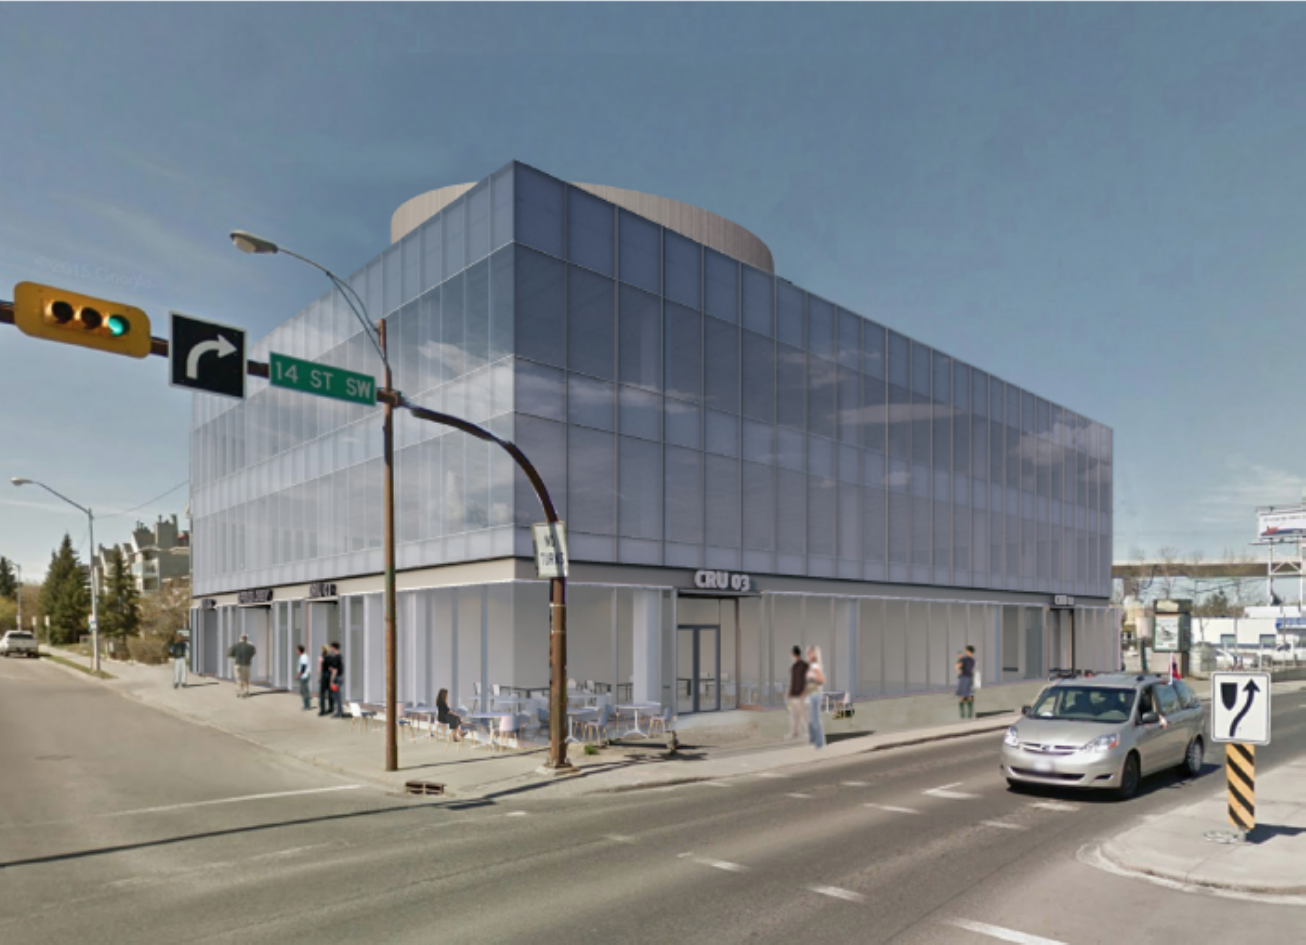
\includegraphics[width = \textwidth]{Assets/CoverPic.png}
    \textbf{Imad Bazzi, 1427883\\Mehuli Das, 1467669\\Ryan Dodyk, 1428580\\Sydney Tarrabain, 1427302\\Hao Zhang, 1425595}

    \huge
    Shiba Structural

    \Large
    April 17, 2019
\end{titlepage}
\section{Introduction}
The purpose of this project is to design a three-storey commercial building located in Vancouver, BC.
The building has the following features:
\begin{itemize}
    \item 1st floor- Mercantile Occupancy
    \item 2nd/3rd floor- Office Occupancy
    \item 2-storey flat slab parkade below grade
    \item Oval-shape enclosure structure on roof for mechanical systems
\end{itemize}
The soil conditions of the site are Class E.
This soil is considered a problem site and would require preloading to consolidate before construction commences.
For this project, our requirements are:
\begin{itemize}
    \item Calculate dead, live due to occupancy, snow, earth pressure, wind and earthquake loads (according to 2015 NBCC Part 4)
    \item Material Selection
    \item Preliminary design options and rationale for final design selection
    \item Design Two-storey parkade:
    \begin{itemize}
        \item Elevator and stair cores
        \item Exterior walls
        \item Columns
        \item Beams
        \item Grid size to satisfy parkade requirements
    \end{itemize}
    \item Design Storeys 1 to 3 and Roof
    \begin{itemize}
        \item Lateral Load Resisting System (LLRS)
        \item Elevator and stairwell cores
        \item Floor system
        \item Columns
        \item Beams
        \item Connections
        \item Grid size
    \end{itemize}
    \item Roof Enclosure
    \begin{itemize}
        \item Wall Assembly
        \item Roof diaphragm
        \item Columns and beams
        \item Connections
    \end{itemize}
    \item Provide Life Cycle Assessment (LCA) of main structural system using Athena Impact Estimator
    \item Innovations
    \item Architectural rendering of building
    \item Structural design calculations for parkade, upper structure, roof enclosure
    \begin{itemize}
        \item Design loading calculation
        \item Load path and method of analysis
        \item Member design
        \item Connection design
        \item Sample calculations
    \end{itemize}
    \item Drawings
    \begin{itemize}
        \item Elevation and plan view drawings with dimensions of structure
        \item Parkade- rebar details, and dimensions of members and assemblies
        \item Upper structure- member sizes, grades and rebar details
        \item Roof enclosure- member sizes and grades
        \item Connections- one typical connection for each “family”
    \end{itemize}
    \item Meeting notes and minutes with mentor/TA
\end{itemize}
\section{Loads}
This section will cover the design loads including dead, live, snow/rain, wind and earthquake loads.
 Our loads are based on 2015 NBCC Part 4 and assumptions based on design elements.
 Also, we assumed out building was located in Vancouver City Hall.
 \subsection{Dead Load}
 The dead loads come from Table 11.25: Mass and weight of materials.
 Assumptions were made about the materials needed for each floor such as protection board, roof membrane, thermal insulation and drywall channel.
\subsubsection{Penthouse Roof}
    \begin{table}[h!]
        \centering
    \begin{tabular}{lcr}
        \toprule
        \textbf{Component} & \textbf{Type} & \textbf{Load (kPa)}\\
        \midrule
        Roof Membrane & 4 ply w/ gravel & 0.32\\
        Protection Board & 14mm thick plywood & 0.08\\
        Thermal Insulation & 75mm rigid glass fibre & 0.53\\
        Drywall Channel & & 0.12\\
        \textbf{Total} & & \textbf{0.58}\\
        \bottomrule
    \end{tabular}
    \caption{Superimposed Penthouse Roof Loads}
    \label{tab:superPent}
    \end{table}

    \begin{table}[h!]
        \centering
    \begin{tabular}{lcr}
        \toprule
        \textbf{Component} & \textbf{Type} & \textbf{Load (kPa)}\\
        \midrule
        Steel Deck & & 0.15\\
        Frame Assumption & & 0.5\\
        \textbf{Total} & & \textbf{0.65}\\
        \bottomrule
    \end{tabular}
    \caption{Penthouse Self Weights}
    \label{tab:selfPent}
    \end{table}

\subsubsection{Mechanical Room Main Roof}
\begin{figure}
    \centering
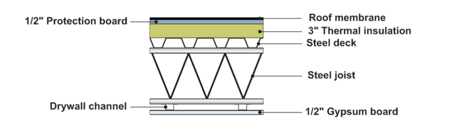
\includegraphics[width=10cm]{Assets/Roof_Structure.png}
\caption{Typical roof detail}
\label{fig:roofStruct}
\end{figure}

\begin{table}[h!]
    \centering
    \begin{tabular}{lcr}
        \toprule
        \textbf{Component} & \textbf{Type} & \textbf{Load (kPa)}\\
        \midrule
        Roof Membrane & 4 ply w/ gravel & 0.32\\
        Protection Board & 14mm thick plywood & 0.08\\
        Thermal Insulation & 75mm rigid glass fibre & 0.053\\
        Drywall Channel &  & 0.12\\
        1/2" Gypsum Board &  & 0.10\\
        Mechanical Piping &  & 0.2\\
        Concrete Equipment Pads & 100mm & 2.35\\
        \textbf{Total} & & \textbf{3.22}\\
        \bottomrule
    \end{tabular}
    \caption{Superimposed main roof loads}
    \label{tab:superMain}
\end{table}

\begin{table}[h!]
    \centering
    \begin{tabular}{lcr}
        \toprule
        \textbf{Component} & \textbf{Type} & \textbf{Load (kPa)}\\
        \midrule
        Composite Deck &  & TBD\\
        Frame Assumption &  & 0.5\\
        \textbf{Total} & & \textbf{TBD}\\
        \bottomrule
    \end{tabular}
    \caption{Superimposed main roof loads}
    \label{tab:selfMain}
\end{table}

We decided to use 100 mm concrete pads, known as “concrete housekeeping pads” (see Figure \ref{fig:Housekeeping_Pads}), for mechanical equipment on the roof.
This is used for cleaning ability in order to spray/wash the floor in case of a spill of a machine without affecting the surrounding machines around.
Also, this also adds extra mass for vibration control.

\begin{figure}
    \centering
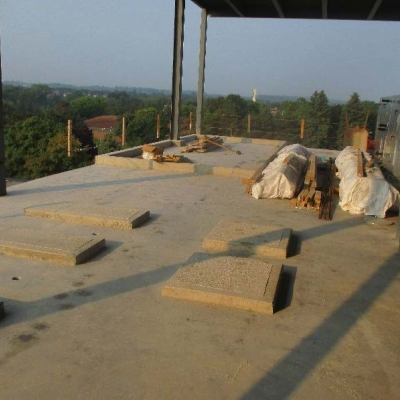
\includegraphics[width=10cm]{Assets/Housekeeping_Pads.png}
\caption{Concrete housekeeping pads}
\label{fig:Housekeeping_Pads}
\end{figure}

\begin{table}[h!]
    \centering
    \begin{tabular}{lcr}
        \toprule
        \textbf{Component} & \textbf{Type} & \textbf{Load (kPa)}\\
        \midrule
        Floor Finishing &  & 0.20\\
        Drywall Channel &  & 0.12\\
        1/2" Gypsum Board &  & 0.10\\
        Partitions &  & 1.00\\
        Mechanical Piping &  & 0.2\\
        \textbf{Total} & & \textbf{1.62}\\
        \bottomrule
    \end{tabular}
    \caption{Superimposed loads on stories 1, 2, and 3}
    \label{tab:super123}
\end{table}

\begin{table}[h!]
    \centering
    \begin{tabular}{lcr}
        \toprule
        \textbf{Component} & \textbf{Type} & \textbf{Load (kPa)}\\
        \midrule
        Composite Deck & P3615 38mm deck w/ 62mm concrete cover & 1.85\\
        Frame Assumption &  & 0.50\\
        \textbf{Total} & & \textbf{2.35}\\
        \bottomrule
    \end{tabular}
    \caption{Self weights of stories 1, 2, and 3}
    \label{tab:self123}
\end{table}

\subsubsection{Parkade Level 1 and 2}

\begin{table}[h!]
    \centering
    \begin{tabular}{lcr}
        \toprule
        \textbf{Component} & \textbf{Type} & \textbf{Load (kPa)}\\
        \midrule
        P1 &  & 0.20\\
        P2 &  & 0.20\\
        \textbf{Total} & & \textbf{0.40}\\
        \bottomrule
    \end{tabular}
    \caption{Superimposed parkade loads}
    \label{tab:superPark}
\end{table}

\begin{table}[h!]
    \centering
    \begin{tabular}{lcr}
        \toprule
        \textbf{Component} & \textbf{Type} & \textbf{Load (kPa)}\\
        \midrule
        RC Slab & 12" & 7162.8\\
        RC Columns & At intersections of beams & 0.61\\
        \textbf{Total} & & \textbf{}\\
        \bottomrule
    \end{tabular}
    \caption{Parkade Self Weights}
    \label{tab:selfPark}
\end{table}

\subsection{Live Load}
The live loads were taken from 2015 NBCC Part 4.1.5.
\subsubsection{Penthouse Roof}
The live load on the penthouse roof is calculated as 1.00 kPa.
This was taken from NBCC 4.1.5.3.
\subsubsection{Mechanical Room Floor}
The live load on the mechanical room floor is calculated as 3.60 kPa.
This was taken from NBCC 4.1.5.3.
\subsubsection{Main Roof}
The live load on the main roof is calculated as 1.00 kPa.
This was taken from NBCC 4.1.5.3.
\subsubsection{Storeys 1, 2, and 3}
The live load on storey 1 is calculated as 4.80 kPa as it is a retail and wholesale area (NBCC 4.1.5.3).
We are designing a slab on the west portion between gridlines C and D of the building of storey 1 (see Figure X) that is capable of withstanding a live load of 12 kPa (NBCC 4.1.5.3). This is designed in anticipation of vehicles driving up on the sidewalk where the parkade lies below grade.

The live load on storeys 2 and 3 is calculated as 2.40 kPa as it is designed for office occupancy. This was taken from NBCC 4.1.5.3.
\subsubsection{Parkade Level 1 and 2}
The live load for parkade levels 1 and 2 is calculated as 2.40 kPa (NBCC 4.1.5.3)  as we assumed vehicles entering the parkade will not exceed 4000 kg gross weight.
Level 1 is also designed for 12.0 kPa on the west portion between gridlines C and D for anticipation of vehicles driving up on the sidewalk.
\subsection{Snow Load}
For detailed calculations of snow loads see Appendix A: Loads.
Specified Snow Load is calculated using the following formula from NBCC 4.1.6.2.1:

\begin{equation*}
    S = I_{s}[S_{s}(C_{b}C_{w}C_{s}C_{a})+S_{r}]
\end{equation*}

\noindent$S_{s} = 1.8 kPa$ (Vancouver City Hall 1/50 NBCC Appendix C)\\
$S_{r} = 0.2 kPa$ (Vancouver City Hall 1/50 NBCC Appendix C)\\
$I_{s} = 1.0 kPa$ (Importance category specified as normal, Table 4.1.6.2)\\
$C_{b} = 0.8$ (NBCC Part 4 Clause 1, Sentence (2)) since $l_{c}=2w-\frac{w^2}{L}=34.6m < 70m$ where $w=30.6$ and $L = 35.2$\\
$C_{w} = 1.0$ (NBCC Part 4 Clause 1, Sentence (3) and (4))\\
$C_{s} = 1.0$ (NBCC Part 4 Clause 1, Sentence (5),(6) and (7))\\

*We assumed the parapet height for the penthouse is 505 mm (same as the roof of Level 3). The detailed drawings did not show the penthouse parapet height.

There are three cases for the accumulation factor ($C_{a}$) :
\begin{enumerate}
\item Upper Roof is source area for snow drift
\item Lower Roof is source area for snow drift (upwind facing step)
\item Lower Roof is source area for snow drift (downwind facing step)
\end{enumerate}

\begin{figure}[h!]
    \centering
    \begin{subfigure}[b]{0.4\linewidth}
        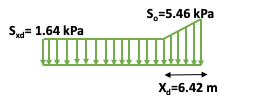
\includegraphics[width=\linewidth]{Assets/case1_snow.png}
        \caption{Case 1, $C_{a}=3.65$}
    \end{subfigure}
    \begin{subfigure}[b]{0.4\linewidth}
        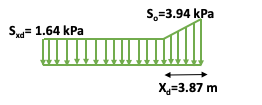
\includegraphics[width=\linewidth]{Assets/case2_snow.png}
        \caption{Case 2, $C_{a}=2.60$}
    \end{subfigure}
    \begin{subfigure}[b]{0.4\linewidth}
        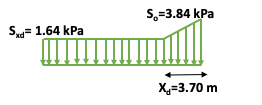
\includegraphics[width=\linewidth]{Assets/case3_snow.png}
        \caption{Case 3, $C_{a}=2.53$}
    \end{subfigure}
    \caption{Snow loads created from different cases}
    \label{fig:snowloads}
\end{figure}

The largest case governs which is case 1 shown in Figure \ref{fig:snowdist} below.
This figure also demonstrates that the penthouse roof has no snow drift as the parapet height of approximately 505 mm is too small to create drift.
Therefore, the snow load on the penthouse roof is 1.64 kPa.

\begin{figure}[h!]
    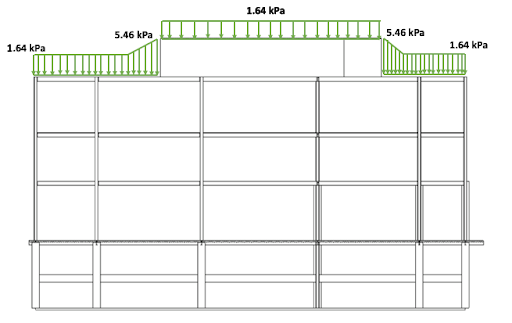
\includegraphics[width=\linewidth]{Assets/snowdist.png}
    \caption{Overall snow load on penthouse and main roof}
    \label{fig:snowdist}
\end{figure}

\subsection{Rain Load}
For the penthouse roof, the rain load is calculated using NBCC Commentary H.
The 24-hr rain period for Vancouver City Hall is 112 mm.
The rain load is calculated as 1.19 kPa.
Therefore, the snow load on the penthouse roof of 1.64 kPa still governs design.
The calculations and assumptions can be found in Appendix A: Loads.

For the main roof, the rain load is calculated using NBCC Commentary H.
The 24-hr rain period for Vancouver City Hall is 112 mm.
The rain load is calculated as 1.15 kPa.
Therefore, the snow load on the main roof of 1.64 kPa still governs design.
The calculations and assumptions can be found in Appendix A: Loads.
\subsection{Wind Load}
\subsubsection{External Pressure}
The wind load is calculated using the static procedure (NBCC 4.1.7.2). The width of the building varies in N-S direction (30.6 m and 33.1 m); however, the larger depth was used for calculations. The building does not require calculations by dynamic or wind tunnel methods as it is a low rise building. The roof enclosure for N-S and E-W, the width will be assumed to be the max width of the enclosure (15.6 m for E-W and 24.0 m for N-S). The roof slope is approximately 0 degrees.

The Specified Wind Load equation found in NBCC 4.1.7.3:

\begin{equation*}
    P=I_{w}qC_{e}C_{g}C_{p}C_{t}
\end{equation*}

$I_{w}= 1.0 kPa$ (assume importance category is normal, Table 4.1.7.1)
$q= 0.45 kPa$ (for Vancouver City Hall)
$C_{t}= 1.0 kPa$
$C_{e}= 0.77$ (stays the same for each level as reference height is less than 20 m)
$C_{g}C_{p}=$ varies for each direction (NBCC Table 4.1.7.6-A)

The following external wind loads are calculated as:
Windward: 0.26 kPa
Leeward: -0.19 kPa
Roof Top (close edge): -0.45 kPa
Roof Top (far edge): -0.24 kPa

The values were calculated assuming that the wind load is applied to the right; if the wind load was applied to the left, the only thing that would change would be that the windward load and the leeward load values would switch with each other, however, the total magnitude would remain the same. As our building has different elevations in different directions; wind loads are designed for the longest dimension (35.2 m) rather than designing wind loads in each direction. Therefore, it was assumed that the building is square with length of 35.2 m on all sides, although this is not the case. Further in detail calculations can be found in Appendix A: Loads.
\subsubsection{Internal Pressure}
The internal wind pressure on the building was calculated as 0 kPa. The internal gust effect factor ($C_{gi}$) is 2.0 kPa (NBCC 4.7.3.10) and the internal pressure coefficient ($C_{pi}$) is 0 kPa (NBCC 4.1.7.7). We assumed through this that the structure is enclosed and any openings will not affect wind loads.

The overall wind pressure can be found in Figure \ref{fig:windload} below.

\begin{figure}[h!]
    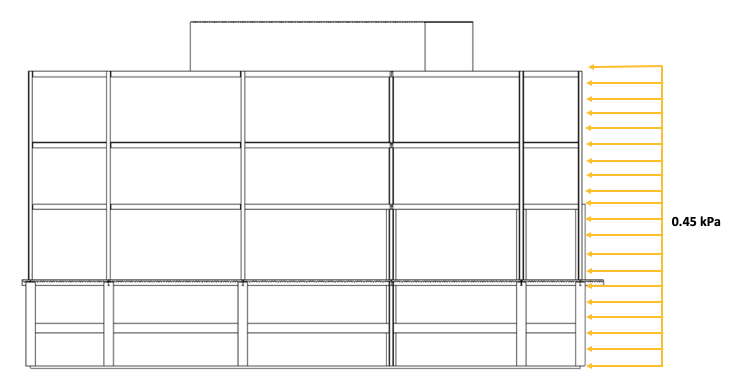
\includegraphics[width=\linewidth]{Assets/windload.png}
    \caption{Overall wind load results}
    \label{fig:windload}
\end{figure}

\subsection{Earthquake Load}
\subsection{Earth Pressure}
\section{Preliminary Design}

\end{document}
